\section{Esercizio 16}
\textit{\textbf{Descrizione:} Scrivere un programma che implementi efficientemente il calcolo di una spline cubica naturale interpolante su una partizione assegnata.}\newline

\noindent\emph{Soluzione: }\newline
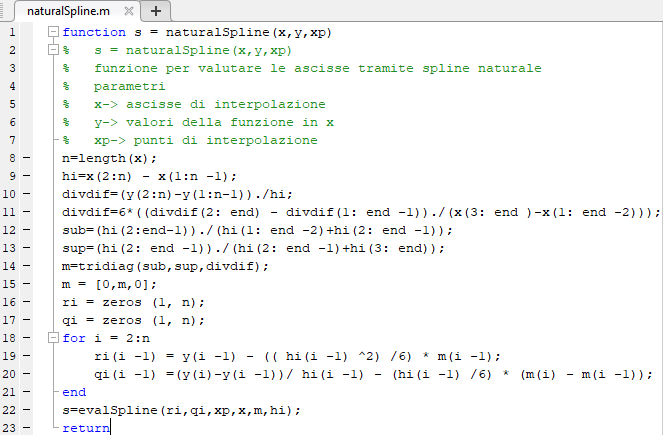
\includegraphics[width=1.3\linewidth]{img/naturalSpline.png}
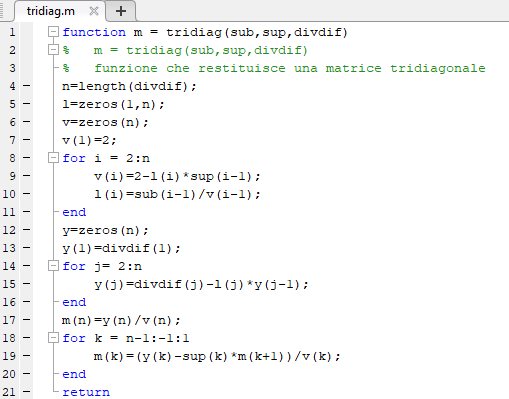
\includegraphics[width=1.3\linewidth]{img/tridiag.png}
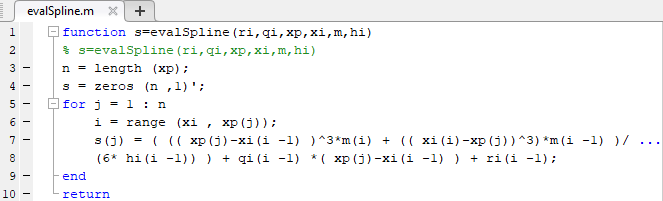
\includegraphics[width=1.3\linewidth]{img/evalSpline.png}
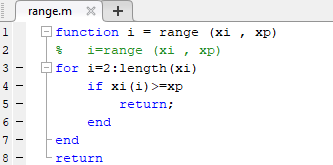
\includegraphics[width=.8\linewidth]{img/range.png}